% Asset ID: A21FunctionsAndGraphsTIKZ-002
% Unit: A21: A2 1 Pure Mathematics
% Topic code: A21-AF
% Related LO IDs: A21-AF-LO006
% Related lesson section: Sketching y = |2x - 3|
% Source: Chapter 2 Functions and Graphs lesson evidence, modulus graph section
% Purpose: Show y = 2x - 3 as a dotted guide and y = |2x - 3| as a reflected graph.

\documentclass[tikz,border=8pt]{standalone}
\usepackage{amsmath}
\usetikzlibrary{arrows.meta}
\begin{document}
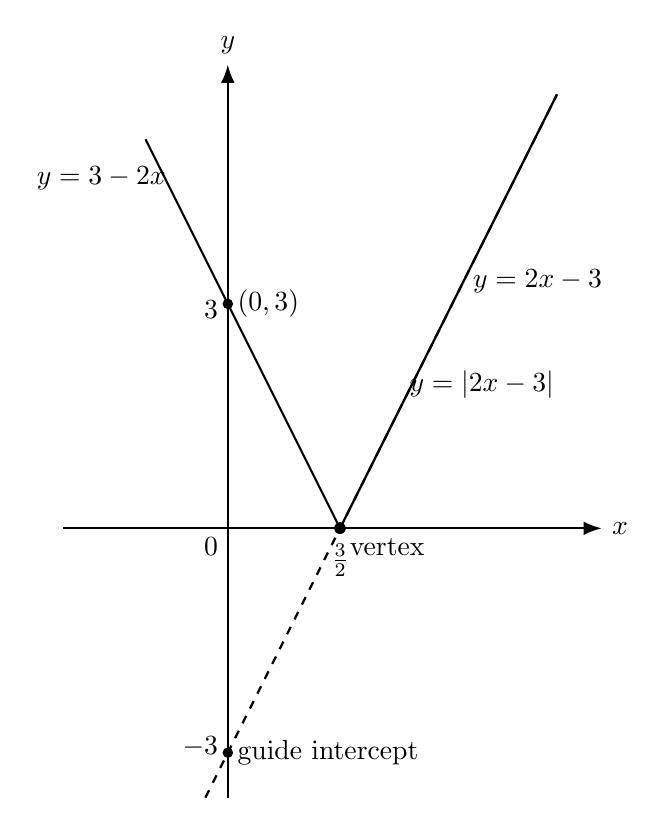
\begin{tikzpicture}[scale=0.95, >=Latex]
\draw[->, thick] (-2.2,0) -- (5,0) node[right] {$x$};
\draw[->, thick] (0,-3.6) -- (0,6.2) node[above] {$y$};
\node[below left] at (0,0) {$0$};
\draw (1.5,0.08) -- (1.5,-0.08) node[below] {$\frac32$};
\draw (0,3.08) -- (0,2.92) node[left] {$3$};
\draw (0,-3.08) -- (0,-2.92) node[left] {$-3$};
\draw[dashed, thick] (-0.3,-3.6) -- (4.4,5.8);
\node[right] at (3.15,3.3) {$y=2x-3$};
\draw[thick] (-1.1,5.2) -- (1.5,0) -- (4.4,5.8);
\fill (1.5,0) circle (2.2pt);
\node[below right] at (1.5,0) {vertex};
\fill (0,3) circle (2pt);
\node[right] at (0,3) {$(0,3)$};
\fill (0,-3) circle (2pt);
\node[right] at (0,-3) {guide intercept};
\node[above left] at (-0.7,4.4) {$y=3-2x$};
\node[above right] at (2.3,1.6) {$y=|2x-3|$};
\end{tikzpicture}
\end{document}
